\documentclass{article}
\usepackage[T1]{fontenc}
\usepackage{template/iclr2027_conference,times}
\usepackage{amsmath,amssymb,graphicx,hyperref,url}
\hypersetup{colorlinks=true,citecolor=blue,urlcolor=blue,linkcolor=blue,
  pdfauthor={Theodore Mui},
  pdftitle={Evaluating JEPA-Inspired Motion Representations Through Geometry and Gait Asymmetry}}
\newcommand{\dg}{^{\circ}}
\iclrfinalcopy
\title{Evaluating JEPA-Inspired Motion\\
Representations Through Geometry\\
and Gait Asymmetry}
\author{Theodore Mui}

\begin{document}
\maketitle
\lhead{Research overview \textbar\ September 2026}


\section{Why pose repair must preserve movement changes}
A future mobility system in the Sequoias study could mistake a knee hidden by furniture for a change in how a resident walks. Such a report could prompt unnecessary concern or obscure a change worth reviewing. Biomechanical assessments face a related problem because estimated joint positions must preserve differences in each leg's movement. This study asks whether repairing noisy poses, which are estimates of joint positions, preserves those movement changes.

To investigate this question, the study uses paired synthetic motions and checks movement changes alongside joint trajectories and correct left--right naming \citep{study2026v08}. The approach draws on joint-embedding predictive architectures (JEPA), which learn numerical features by predicting reference features. Earlier work applied this idea to recognizing actions from joint motion \citep{abdelfattah2024sjepa}. Here, the focus is gait asymmetry, or differences between the legs. The experiments did not evaluate Sequoias residents, balance tasks, or fall outcomes.

\section{A controlled movement and observation test}
Walking candidates are selected from AMASS recordings of 3D body motion \citep{mahmood2019amass} using filenames and the geometry of joints mapped into camera images. The training pool contains 112 people, 692 motions, and 1,645 short clips, called windows. Although the paper omits the training subsets, saved records identify BioMotionLab\_NTroje, KIT, Eyes\_Japan\_Dataset, and ACCAD. Methods are compared on 155 development clips from 14 different people, including 12 from BioMotionLab\_NTroje and two from KIT. Their clinical status is not established.

Each roughly five-second clip has 128 samples at 25 samples per second. An ankle-height rule activates right-knee rotations of $0,5,10,15\dg$, which fade at clip boundaries. After editing, the body may be reflected with its sides exchanged. Synthetic images show angled ($45\dg$) or side ($90\dg$) views, sometimes partly covered by an artificial blocker. RTMPose-M, HRNet-W32, and ViTPose-base estimate poses from known person locations, excluding errors in finding the person. To test naming errors separately, estimated left--right joint names are exchanged throughout a clip or its middle third while reference names stay fixed. These manipulations do not simulate disease or a furnished room.

Variants of known people and duplicate motions stay within their assigned data split. The $15\dg$ edit and ViTPose are withheld during training and selection of loss strengths, but evaluated on the same development people. Reserved test participants were not evaluated. Unrecognized duplicate identities or overlap with pose estimators' earlier training remain possible.

\begin{figure}[!htb]
\begin{minipage}[c]{0.47\linewidth}
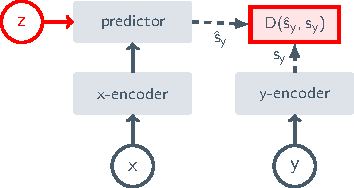
\includegraphics[width=\linewidth]{assets/external/vjepa-figure2.pdf}
\end{minipage}\hfill
\begin{minipage}[c]{0.50\linewidth}
\caption{\textbf{External JEPA concept.} Encoders turn inputs $x,y$ into numerical features. The predictor estimates $y$'s features using $z$, which describes how $y$ is formed. The function $D$ measures feature mismatch. Reproduced unchanged from \citet{bardes2024vjepa}, Fig.~2, under \href{https://creativecommons.org/licenses/by/4.0/}{CC BY 4.0}. In v08, the inputs are joint sequences, and clean synthetic reference poses are available only during training.}
\label{fig:concept}
\end{minipage}
\end{figure}

\clearpage
\section{How the model learns and what is measured}
The student encoder converts 12 joints' noisy 2D positions, estimator scores, missing-data flags, and times into features. Positions are first shifted and rescaled using available observations. Groups of four samples per joint feed a four-layer transformer that combines information across joints and time. During pretraining, the initial feature-learning stage, selected joints and time spans are hidden. A predictor learns reference features from a teacher that sees clean projected joints and follows a weighted running average of student parameters. Cross-entropy compares teacher and predicted feature probabilities, while other penalties discourage identical features across clips. Training therefore uses \emph{clean synthetic reference poses available only during training}. Access to complete clips allows restoration without testing future prediction.

Two additional losses, or training-error terms, test what the features preserve. The \textbf{per-sequence feature-matching loss} compares predicted and teacher features separately for the original clip and its edited partner. The \textbf{paired feature-change loss} instead compares the student's edited-minus-original feature difference with the teacher's corresponding difference. Because shared errors cancel in subtraction, two inaccurate predictions can still produce the right difference. Neither loss directly measures knee angles. The figure labels these ``endpoint'' and ``delta,'' where an endpoint is a clip rather than its first or last frame.

A small output network called a readout converts features to coordinates. After 2,000 pretraining updates, the encoder stays fixed, or frozen, for 2,000 readout updates. Direct training updates both networks for 4,000 steps, so encoder training differs despite equal totals.

\paragraph{What counts as preserving change?}
Knee-angle excursion is the range between the 5th and 95th percentiles within each clip, excluding extremes. Asymmetry is right minus left excursion, and its change between paired clips is the ``response.'' Response error measures the absolute difference from the reference change. Waveform error averages absolute knee-angle errors across legs and time. Localization error divides position error by the diagonal of the person's image box, while naming checks count wrong, ambiguous, or missing side assignments. These 2D measurements do not establish 3D anatomical accuracy. Where references permit measurement, invalid predictions incur worst-case costs of $720\dg$ for response and $180\dg$ for waveforms. Scores are averaged in stages over clips, motions, people, and three training runs, with seeds controlling each run's random choices.

\begin{figure}[!htb]
\centering
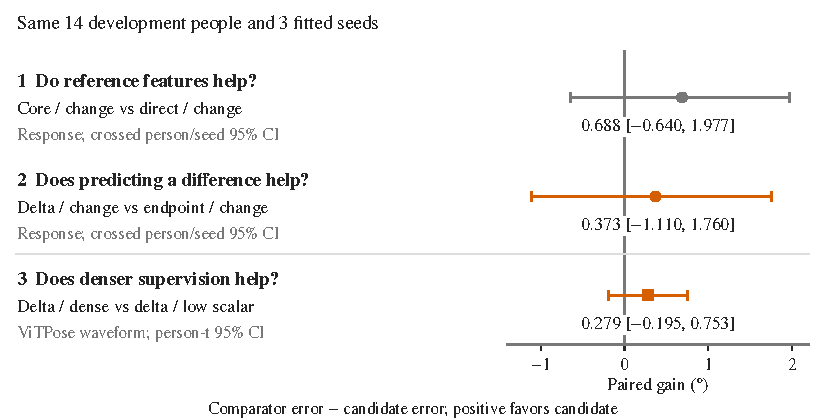
\includegraphics[width=\linewidth]{assets/v08-study-questions.pdf}
\caption{\textbf{Three uncertain comparisons.} Reproduced unchanged from v08, Fig.~7. Positive gains mean lower error, but all 95\% confidence intervals (CI) span gains and losses. ``Crossed'' bootstrap resamples people and training runs separately; ``person-$t$'' uses variation across people after averaging runs. ``Core'' denotes the base JEPA model. Both first-row methods add the change penalties explained on page~3, so this comparison excludes the stronger coordinate-only baseline.}
\label{fig:results}
\end{figure}

\clearpage
\section{What improved and what remains unresolved}
Training directly against clean coordinates improves waveform error from $18.57\dg$ to $12.07\dg$ and response error from $12.69\dg$ to $7.54\dg$ relative to unchanged inputs. The exploratory estimate of this response gain is $5.14\dg$, with a 95\% interval of [2.15, 8.65]. Yet always predicting zero change gives $5.81\dg$ response error, below all 16 trained variants. Although scoring excludes zero-edit pairs, small projected changes, estimation errors, and failed reconstructions affect the comparison. Zero prediction produces no trajectory, and its advantage does not rule out useful change information in the features.

An exploratory analysis finds that direct coordinate training beats zero response for all 14 development people in clear images, but only one with blocked visibility, or occlusion. An ambient system would therefore need to check whether reported mobility changes persist across visibility conditions. The synthetic blocker cannot establish how often this problem occurs in a residence.

Figure~\ref{fig:results} also leaves JEPA's benefit over direct training and the difference between the two feature losses unresolved. Different initial contributions to the signal for updating parameters, along with separately evolving teachers, complicate this comparison. The original ``change'' readout adds penalties for asymmetry-change error and excessively short predicted limb segments to coordinate error. Together, these worsen waveform error in all eight model families, although their individual effects are not isolated. On ViTPose, the feature-change model's waveform error falls from $23.17\dg$ to $19.47\dg$ when the single-number response penalty receives less weight (``low scalar''). Supervising angle changes for each leg and timestamp (``dense'') brings the error to $19.19\dg$, but the added benefit remains uncertain. A single response can hide timing errors or errors that cancel between legs, making waveform and naming checks important.

Controls include untrained encoders, incorrect reference pairings, and pretraining to predict coordinates. Published pose-repair models such as MotionBERT \citep{zhu2023motionbert} were not evaluated. The uncertainty intervals also omit the effects of using development results to guide later experiments. Synthetic references cannot establish natural-video performance, and missing predictions and saved parameters prevent full replication. The study does not validate asymmetry as a balance or fall-risk outcome.

\section{Proposed next study: checking movement comparisons}
A follow-up study could search for joint trajectories that fit visible observations equally well but imply different changes in each leg. Finding such alternatives would reveal ambiguity in the movement estimate. Related work already covers selecting biomechanical measurements by uncertainty \citep{pace2026uncertainty}, single-camera reconstruction \citep{gilon2026opencap}, and JEPA-pretrained gait estimation under occlusion \citep{mehraban2026synthgait}. The question is whether this search identifies misleading comparisons better than simpler uncertainty rules.

A pilot could use two walking trials per person with known camera geometry and simultaneous motion capture using body-mounted markers. Intended changes must exceed reference measurement uncertainty in at least one leg's 3D knee excursion. Clear and digitally blocked copies of one trial provide no-change controls, while separate trials provide measured changes. With camera and body dimensions fixed within each pair, the same repair model would receive identical coordinate training with or without JEPA pretraining. Comparisons would include zero-change prediction and interpolation, which fills gaps from neighboring frames. The search would be compared with visibility rules, error ranges adjusted against held-out references, and disagreement among independently trained models. Joint-angle limits must allow asymmetric movement.

Training, setting error ranges, and final testing would use different people. Success requires preserving each leg's measured change and reducing false, missed, or wrong-side changes at equal reporting rates for \emph{whole trial pairs}. Repeated reference measurements would set tolerances, with uncertainty assessed across people and the analysis showing whose measurements are withheld. Anatomical assumptions could suppress atypical gait, and a limited search could miss valid alternatives. For Landay's lab, this could support inconclusive reports or requests for another observation. Delp's lab could test whether movement differences survive reconstruction before extending to balance assessments.

\clearpage
\bibliography{references}
\bibliographystyle{template/iclr2027_conference}
\end{document}
